% ============================================================
%  深圳大学实验报告模板（SZU Experiment Report Template）
%  Produced by: Chao Fan and Kewei Ou, AI School of SZU
%  仅按本项目内容填充正文，封面、章节框架与批阅页保持模板原样。
% ============================================================

\documentclass[a4paper,12pt]{article}

% ----------------------------
% 中文与字体支持（Overleaf 用 Noto Serif CJK SC，本机改用宋体）
% ----------------------------
\usepackage{fontspec}
\usepackage{xeCJK}
\setCJKmainfont[AutoFakeBold=2]{SimSun}

% ----------------------------
% 页面设置与常用宏包
% ----------------------------
\usepackage{geometry}
\geometry{left=1in, right=1in, top=0.85in, bottom=0.85in}
\usepackage{longtable}
\usepackage{graphicx}
\usepackage{fancyhdr}
\usepackage{tikz}
\usetikzlibrary{calc}
\usepackage{verbatim}
\usepackage{float}
\usepackage{array}
\usepackage{url}

\linespread{0.94}
\setlength{\parskip}{2pt plus 1pt minus 1pt}
\setlength{\itemsep}{0pt}
\setlength{\floatsep}{6pt}
\setlength{\textfloatsep}{6pt}
\setlength{\intextsep}{4pt}
\renewcommand{\arraystretch}{1.05}
\renewcommand{\figurename}{图}

\fancyhf{}
\fancyhead[C]{}
\fancyhead[R]{}

\begin{document}

% ============================================================
% 封面页（按官方模板原样）
% ============================================================
\begin{titlepage}
    \centering
    \vspace*{2cm}
    \Huge{\textbf{深 \ 圳 \ 大 \ 学 \ 实 \ 验  \ 报 \ 告}}\\[1.5cm]

    {\Large\textbf{课程名称}\quad\underline{\makebox[8cm][c]{Python程序设计}}}\\[0.5cm]
{\Large
\noindent\makebox[3.2cm][l]{\textbf{项目名称}}
\underline{\makebox[8cm][c]{Project 1 NumPy 图像编码器}}}\\[0.5cm]
{\Large
\noindent\makebox[3.2cm][l]{\textbf{学 \quad \quad 院}}
\underline{\makebox[8cm][c]{人工智能学院}}}\\[0.5cm]
{\Large
\noindent\makebox[3.2cm][l]{\textbf{专 \quad \quad 业}}
\underline{\makebox[8cm][c]{}}}\\[0.5cm]
{\Large
\noindent\makebox[3.2cm][l]{\textbf{指导教师}}
\underline{\makebox[8cm][c]{舒婷}}}\\[0.5cm]
{\Large
\noindent\makebox[3.2cm][l]{\textbf{报 \quad 告 \quad 人}}
\underline{\makebox[3cm][c]{}}
\hspace{0.5cm}
\textbf{学号}
\underline{\makebox[3cm][c]{}}}\\[0.5cm]
{\Large
\noindent\makebox[3.2cm][l]{\textbf{实验时间}}
\underline{\makebox[8cm][c]{2026 年 11 月}}}\\[0.5cm]
{\Large
\noindent\makebox[3.2cm][l]{\textbf{提交时间}}
\underline{\makebox[8cm][c]{2026 年 11 月 26 日}}}\\[1.5cm]

    \vfill
    \Large{\textbf{教务处制}}
\end{titlepage}

\newpage

% ============================================================
% 正文部分
% ============================================================

\section{实验目标与方法 (Objectives / Overview)}

\textbf{目标}：给定图像与训练好的参数，不用深度学习框架，仅用 NumPy 手写 ViT-B-32 图像塔前向计算，把每张图编码为 512 维单位长度特征，并与独立的 Torch FP32 参考逐阶段对齐；不训练、不把参考数组当作输入。输入为 10 张图片与 \texttt{weights/image\_encoder.npz} 参数，输出为 \texttt{results/output\_tokens.npz}（形状 $10\times512$，float32）。

\begin{table}[H]
\centering\small
\begin{tabular}{|l|l|p{5.4cm}|}
\hline
环节 & 输入 $\to$ 输出 & 关键运算 \\
\hline
预处理（提供） & 图片 $\to$ [B,3,224,224] & 双三次最短边缩放、中心裁剪、逐通道标准化 \\
patchify（01） & $\to$ [B,49,3072] & $7\times7$ 网格重排，块内 C,H,W 展开 \\
embed（05） & $\to$ [B,50,768] & 无偏置 patch 投影、前置 CLS、加位置向量 \\
12 层 Block（02/03/04） & $\to$ [B,50,768] & LayerNorm、12 头注意力、精确 GELU MLP、两条残差 \\
输出头（06） & $\to$ [B,512] & 取 CLS、ln\_post、visual.proj、单位化 \\
\hline
\end{tabular}
\end{table}

\begin{figure}[H]
\centering
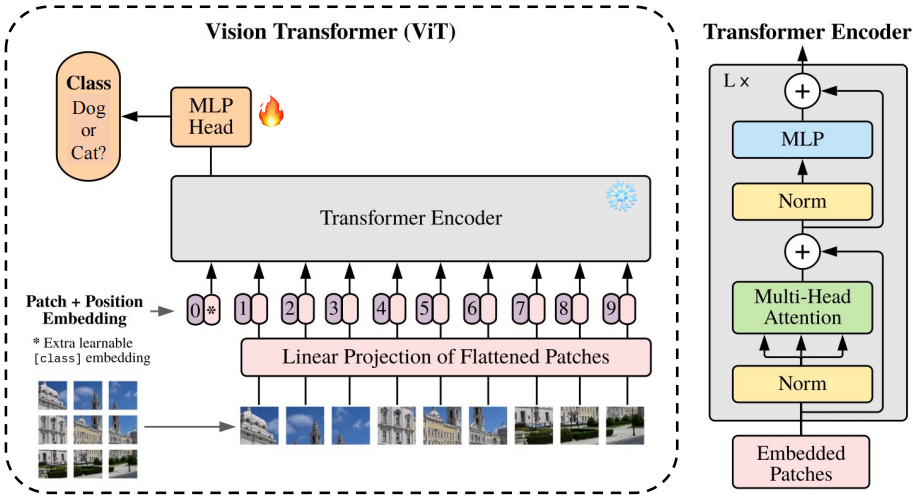
\includegraphics[width=0.62\linewidth]{figs/vit_overview.png}
\caption{ViT 图像塔结构：切块线性投影、位置嵌入、L 层 Transformer Encoder、CLS 经 MLP Head 输出（模板示例图）}
\end{figure}

\textbf{本人贡献}：独立完成 6 组 TODO 的实现与 shape 推导、逐阶段排查、8 项数值校验、输出特征导出、误差表与图、README、本报告及提交说明。课程提供的 \texttt{helpers.py}、\texttt{preprocess\_image.py}、\texttt{runtime.py}、\texttt{run.py}、\texttt{check.py}、\texttt{transformer\_steps.py} 及权重/图片/manifest 均未改动；课件与 \texttt{PPT-CODE-MAP.txt} 用于确认计算顺序，AI 助手仅审阅代码与润色排版。

\section{实现要点 (Implementations)}

以课件 39--73 页和 \texttt{transformer\_steps.py} 迷你示例为依据，按张量形状自行推导多头组织。\texttt{split\_heads}: [B,N,768] $\to$ reshape(B,N,12,64) $\to$ transpose(0,2,1,3) $\to$ [B,12,N,64]；合并为其严格逆操作。注意力分数 $\mathrm{softmax}(qk^\top/\sqrt{64})v$，其中 k 为 4D，只能交换最后两轴 \texttt{k.transpose(0,1,3,2)}，不能照搬 2D 示例写 \texttt{k.T}。两处易错点：其余线性权重为 [out,in] 需用 W.T，唯 \texttt{visual.proj} 已是 [in,out]=[768,512]（由 \texttt{config.json} 的 \texttt{output\_projection\_layout} 确认）；第一条残差必须加在原始 x 而非 norm1(x)。LayerNorm 用 eps=1e-5，GELU 用精确 erf 形式，与 Torch 保持一致。

\section{环境、参数与可复现性 (Reproducibility)}

\textbf{环境}：Windows 11、Python 3.14.3、NumPy 2.4.3、Pillow 12.3.0；无 GPU、无 PyTorch、无 OpenCLIP、无联网。依赖见 \texttt{requirements.txt}：numpy 1.24 及以上、3 以下；Pillow 9.2 及以上、13 以下；imageio 2.31 及以上、3 以下，安装命令 \texttt{python -m pip install -r requirements.txt}。

\textbf{关键参数}：输入 $224\times224$ RGB float32；patch $32\times32$，共 $7\times7=49$ 个，展平 3072 维；width 768 / heads 12 / head\_dim 64 / layers 12 / MLP 3072；序列 CLS + 49 patch = 50 token；输出 512 维且 L2 范数为 1；归一化 mean=(0.48145466, 0.4578275, 0.40821073)，std=(0.26862954, 0.26130258, 0.27577711)。

\textbf{数据获取}：仓库含 10 张图片（约 412 KB）、\texttt{config.json}、\texttt{images.json} 与两个 manifest.json。权重 \texttt{weights/image\_encoder.npz}（约 311 MiB / 152 个张量）与 \texttt{assets/reference\_outputs.npz}（约 7.3 MiB）超过 GitHub 单文件 100 MB 上限，按 README 第 3 节从课程附件复制回对应目录，\texttt{check.py --stage assets} 自动校验 SHA-256；参考输出只被 check.py 读取。

\textbf{运行步骤}（仓库根目录，\texttt{--stage all} 实测约 2 分 13 秒）：
\begin{verbatim}
python -m pip install -r requirements.txt
python transformer_steps.py
python check.py --stage assets
python check.py --stage all
python run.py --output results/output_tokens.npz
\end{verbatim}
\textbf{判定}：shape 一致、float32、有限值，且 abs(actual$-$reference) $\le$ atol + rtol$\cdot$abs(reference)；atol：output/batch 2e-5、内部 token 2e-4、preprocess 2e-6，rtol=2e-4；输出每行范数为 1。

\section{结果与证据 (Results)}

\begin{table}[H]
\centering\small
\begin{tabular}{|l|l|r|r|r|l|}
\hline
阶段 & shape & max\_abs & mean\_abs & atol & 结论 \\
\hline
preprocess & (10,3,224,224) & 0.000e+00 & 0.000e+00 & 2e-6 & PASS \\
patches & (2,49,3072) & 0.000e+00 & 0.000e+00 & 2e-4 & PASS \\
tokens & (2,50,768) & 4.005e-05 & 1.289e-06 & 2e-4 & PASS \\
block0 & (2,50,768) & 7.063e-06 & 3.250e-07 & 2e-4 & PASS \\
last\_tokens & (2,50,768) & 4.768e-05 & 2.696e-06 & 2e-4 & PASS \\
output & (10,512) & 5.439e-07 & 8.306e-08 & 2e-5 & PASS \\
batch & (3,512) & 4.619e-07 & 7.632e-08 & 2e-5 & PASS \\
\hline
\end{tabular}
\end{table}

全部 8 阶段 PASS。preprocess 与 patches 逐位相同；中间 token 最大误差 4.768e-05，最终输出最大误差 5.439e-07，约为容差 2e-5 的 $1/37$。batch 使用 [1,0,1] 乱序加重复输入同样通过。

\begin{figure}[H]
\centering
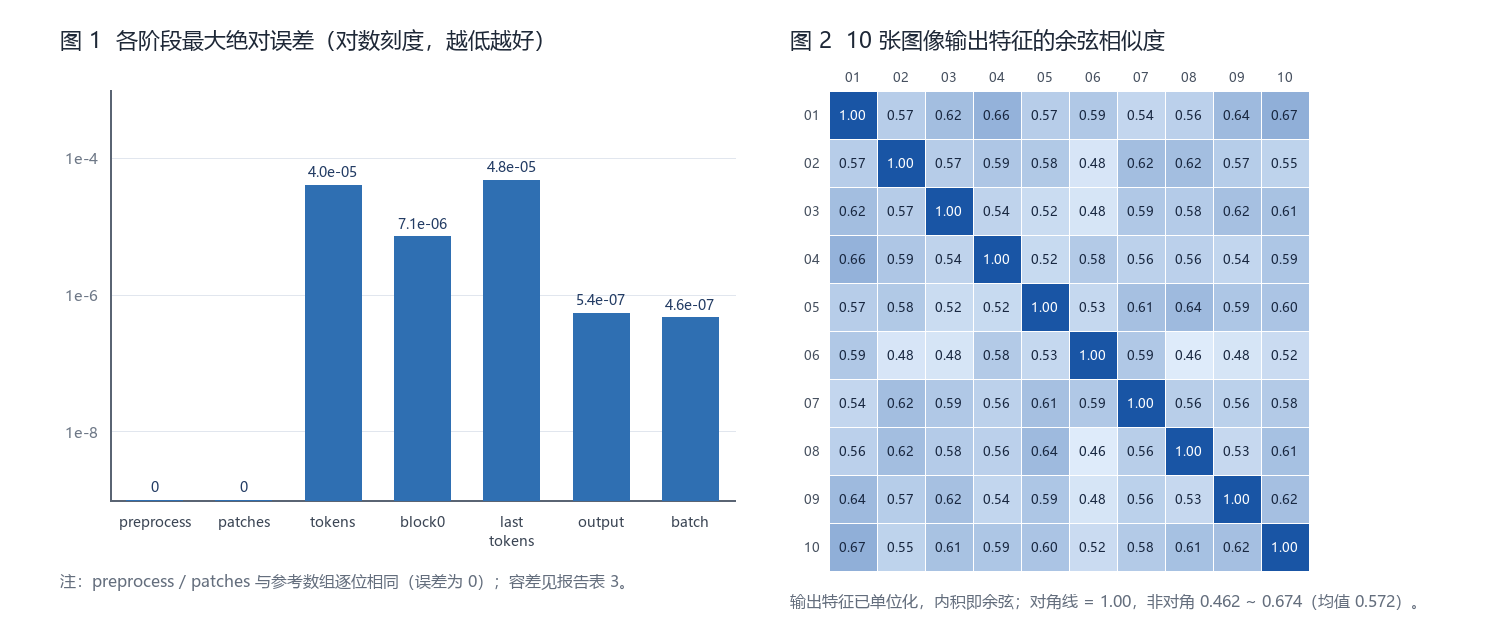
\includegraphics[width=0.90\linewidth]{figs/evidence_figure.png}
\caption{左：各阶段最大绝对误差（对数刻度）与容差；右：10 张图输出特征的 $10\times10$ 余弦相似度热力图}
\end{figure}

\textbf{关键输出}：\texttt{output\_tokens} 形状 (10,512)、float32，每行范数 1.000000；image\_01 前 6 个分量 [-0.039898, +0.085013, +0.079881, +0.021347, +0.021042, +0.000435]。\texttt{results/similarity.csv} 对角线为 1.000，非对角 0.462--0.674（均值 0.572），说明不同图像的特征可区分。\textbf{结论}：纯 NumPy 前向与独立 Torch FP32 参考在全部中间阶段及最终输出一致，误差远小于容差，单位化、批量乱序与重复图等边界行为均通过。

\section{分析与反思 (Discussion)}

\textbf{解释与比较}：误差主要来自矩阵乘累加顺序与 float32 舍入（中间阶段约 1e-5），经 ln\_post、投影与单位化后回落到约 5e-7，未被 12 层放大；preprocess/patches 为 0，因为前者由课程代码提供、后者只是纯重排。相比直接调用 PyTorch，NumPy 逐层展开便于核对 shape 与定位误差来源，代价是速度较慢。

\textbf{失败与修复}：本机初始仅有 NumPy，首次运行 \texttt{check.py} 在 \texttt{load\_images()} 处报 \texttt{ModuleNotFoundError: No module named 'PIL'}；按 requirements.txt 补装 Pillow 12.3.0 后 8 阶段一次通过。数值校验本身未出现 FAIL，得益于按阶段逐个排查而非一次性全量比对。

\textbf{局限与改进}：（1）\texttt{helpers.GELU} 用 Python 循环逐元素 math.erf，全量校验约 2 分 13 秒，可改向量化 erf 并做等价性对照；（2）326 MB 权重超 GitHub 单文件上限，已在 README 写明获取方法与 SHA-256 校验，必要时用 Git LFS；（3）仅图像塔、参数固定，无文本塔/训练/下游评测，后续可做跨模态检索；（4）注意力矩阵 [B,12,50,50] 内存随 B 线性增长，大批量可分块。

\textbf{提交信息}：GitHub 地址为 Public 仓库，助教与老师可直接访问：\\
{\small\url{https://github.com/szu-maze-runner/project1-numpy-image-encoder}}\\
仓库含源码、README.md、requirements.txt、小数据、results/、report/，保留多次真实 commit，未 squash 或 force push。报告正文控制在 5 页以内。

\newpage

% ============================================================
% 批阅与成绩评定页（按官方模板原样保留）
% ============================================================

\begin{tikzpicture}[remember picture, overlay]
  \draw[thick]
    ($(current page.north west)+(2cm,-3cm)$)
    rectangle
    ($(current page.south east)+(-2cm,3.5cm)$);
\end{tikzpicture}

\vspace{1cm}

\noindent \textbf{指导教师批阅意见：}
\vspace{6cm}
\hfill

\vspace{1cm}

\noindent \textbf{成绩评定：}
\vspace{2cm}
\hfill

\vspace{1cm}

\noindent
\hfill
\textbf{指导教师签字：}\quad\quad\quad\quad\quad\\[0.5cm]

\hfill
\textbf{年}\quad\quad
\textbf{月}\quad\quad
\textbf{日}\quad

\vspace{1cm}

\noindent \textbf{备注：}

\begin{tikzpicture}[remember picture, overlay]
  \node[
    anchor=north west,
    inner sep=0pt,
    text width=\dimexpr\paperwidth-4cm\relax
  ] at ($(current page.south west)+(2cm,3.1cm)$) {
    \begin{minipage}{\dimexpr\paperwidth-4cm\relax}
      \small
      \noindent
      \textbf{注：}\;1、报告内的项目或内容设置，可根据实际情况加以调整和补充。\\[0.2cm]
      \phantom{\textbf{注：}\;}2、教师批改学生实验报告时间应在学生提交实验报告时间后 10 日内。
    \end{minipage}
  };
\end{tikzpicture}

\end{document}
